%%
%% Automatically generated file from DocOnce source
%% (https://github.com/hplgit/doconce/)
%%
%%


%-------------------- begin preamble ----------------------

\documentclass[%
oneside,                 % oneside: electronic viewing, twoside: printing
final,                   % draft: marks overfull hboxes, figures with paths
10pt]{article}

\listfiles               %  print all files needed to compile this document
\usepackage{mathtools}
\usepackage{relsize,makeidx,color,setspace,amsmath,amsfonts,amssymb}
\usepackage[table]{xcolor}
\usepackage{bm,ltablex,microtype}
\usepackage{float}
\usepackage[pdftex]{graphicx}
\usepackage{epstopdf}
\usepackage{verbatim}

\usepackage{fancyvrb} % packages needed for verbatim environments

\usepackage[T1]{fontenc}
%\usepackage[latin1]{inputenc}
\usepackage{ucs}
\usepackage[utf8x]{inputenc}
\usepackage[english]{babel}
\usepackage{lmodern}         % Latin Modern fonts derived from Computer Modern

% Hyperlinks in PDF:
\definecolor{linkcolor}{rgb}{0,0,0.4}
\usepackage{hyperref}
\hypersetup{
    breaklinks=true,
    colorlinks=true,
    linkcolor=linkcolor,
    urlcolor=linkcolor,
    citecolor=black,
    filecolor=black,
    %filecolor=blue,
    pdfmenubar=true,
    pdftoolbar=true,
    bookmarksdepth=3   % Uncomment (and tweak) for PDF bookmarks with more levels than the TOC
    }
%\hyperbaseurl{}   % hyperlinks are relative to this root

\setcounter{tocdepth}{2}  % levels in table of contents



% prevent orhpans and widows
\clubpenalty = 10000
\widowpenalty = 10000

% --- end of standard preamble for documents ---


% insert custom LaTeX commands...

\raggedbottom
\makeindex
\usepackage[totoc]{idxlayout}   % for index in the toc
\usepackage[nottoc]{tocbibind}  % for references/bibliography in the toc

%-------------------- end preamble ----------------------

\begin{document}

% matching end for #ifdef PREAMBLE

\newcommand{\exercisesection}[1]{\subsection*{#1}}


% ------------------- main content ----------------------



% ----------------- title -------------------------

\thispagestyle{empty}

\begin{center}
{\LARGE\bf
\begin{spacing}{1.25}
PHYS 905 - Project 2
\end{spacing}
}
\end{center}

% ----------------- author(s) -------------------------

\begin{center}
{\bf Terri Poxon-Pearson}
\end{center}

    
% ----------------- end author(s) -------------------------

% --- begin date ---
\begin{center}
February 27, 2017
\end{center}
% --- end date ---

\vspace{1cm}

In this report we implement Jacobi's Algorithm to solve Shroedinger's equation for electrons in a harmonic oscillator.  We first explore the case of a single electron and are able to reproduce the lowest eigenvalues to high accuracy.  Next we explore the case of two interacting electrons in the oscillator.  For an oscillator frequency of $\omega = 0.25$ we are able to reproduce the lowest eigenvalue of 1.2499 which can be found analytically.  Jacobi's method also provides easy access to eigenvectors.  Studying these wave functions gives physical insight into the two-electron system.

\tableofcontents
 
\section{Introduction}
In this project we will be solving Schroedinger's equation for the case of electrons in a 3D harmonic oscillator. First, we will first solve the simpler, non-interacting case with just one electron in the harmonic oscillator potential using Jacobi's method. Next, we will add a second electron with interacts via a repulsive, Coulomb potential.  This will involve a change into center of mass coordinates.  Both problems will be solved for l=0 case.  Additionally, we will explore our calculation's sensitivity to parameters such as the number of mesh points and maximum integration radius.

This report will begin with a brief introduction to the physical system we are studying in this project, as well as a description of how these equations are discretized.  Next we will describe the method used to solve this eigenvalue problem.  We will discuss the implementation of this algorithm, including a discussion of sensitivity to various integration variables and tests used to check the code's validity.  Finally, I will present the results of my calculations, followed by some conclusions.
\section{Methods}

\subsection{Physics of Single Electron in 3D Oscillator}

If we assume spherical symmetry, the radial part of Shroedinger's equation for a single electron in a harmonic oscillator can be writen as

\begin{equation*}
  -\frac{\hbar^2}{2 m} \left ( \frac{1}{r^2} \frac{d}{dr} r^2
  \frac{d}{dr} - \frac{l (l + 1)}{r^2} \right )R(r) 
     + V(r) R(r) = E R(r).
\end{equation*}

where $V(r)$ is the harmonic oscillator potential.  The energies $E$ for the 3D harmonic oscilator are well know and given by

\begin{equation*}
E_{nl}=  \hbar \omega \left(2n+l+\frac{3}{2}\right).
\end{equation*}

To simplify the expression, we can make the common substitution $R(r) = (1/r) u(r)$, leaving us with
% 

\begin{equation*}
  -\frac{\hbar^2}{2 m} \frac{d^2}{dr^2} u(r) 
       + \left ( V(r) + \frac{l (l + 1)}{r^2}\frac{\hbar^2}{2 m}
                                    \right ) u(r)  = E u(r) .
\end{equation*}
% 

We have two boundary conditions to constrain this differential equations.  First, we want the wave function to disappear at the origin, so $u(0)=0$.  Second, the wave function should be localized to the oscillator well, so we want $u(\infty)=0$.  Here, we will only consider $l=0$ states, which eliminates one term of the equation.  Finally, we can introduce a dimensionless variable $\rho = (1/\alpha) r$ and insert  $V(\rho) = (1/2) k \alpha^2\rho^2$, leaving us with

\begin{equation*}
  -\frac{\hbar^2}{2 m \alpha^2} \frac{d^2}{d\rho^2} u(\rho) 
       + \frac{k}{2} \alpha^2\rho^2u(\rho)  = E u(\rho) .
\end{equation*}

Multiplying through my the leading factors leaves us with

\begin{equation*}
  -\frac{d^2}{d\rho^2} u(\rho) 
       + \frac{mk}{\hbar^2} \alpha^4\rho^2u(\rho)  = \frac{2m\alpha^2}{\hbar^2}E u(\rho) .
\end{equation*}

Now we can choose that

\begin{equation*}
\frac{mk}{\hbar^2} \alpha^4 = 1
\end{equation*}

and define

\begin{equation*}
\lambda = \frac{2m\alpha^2}{\hbar^2}E.
\end{equation*}

That leaves us with the final expression

\begin{equation*}
  -\frac{d^2}{d\rho^2} u(\rho) + \rho^2u(\rho)  = \lambda u(\rho) .
\end{equation*}

This is the equation that we must solve numerically.  There are analytic solutions in the case of $l=0$ and the three lowest eigenvalues are $\lambda_0=3,\lambda_1=7,\lambda_2=11$. We can compare the accuracy of our results to these exact solutions.

\subsection{Discretization of Schroedinger's Equation}

As in Project 1, we will discretize the differential equation and use the three point formula to express the second derivative.  This expression is given by
 
\begin{equation*}
    u''=\frac{u(\rho+h) -2u(\rho) +u(\rho-h)}{h^2} +O(h^2).
    \label{eq:diffoperation}
\end{equation*}

A full derivation of this expression can be found in \cite{LectureNotes}.  Here, $h$ is the step size where 

\begin{equation*}
  h=\frac{\rho_N-\rho_0 }{N}
\end{equation*}

and the value of $\rho$ at a point $i$ is then 

\[
    \rho_i= \rho_0 + ih \hspace{1cm} i=1,2,\dots , N.
\]

$N$ defines the number of grid points. Because this is a radial integral, the define minimum value for $\rho$ is 0 and  $\rho_{\mathrm{max}}=\rho_N$,

Using the compact notation from project one, we can rewrite the Schroedinger equation as

\[
-\frac{u_{i+1} -2u_i +u_{i-1}}{h^2}+\rho_i^2u_i=-\frac{u_{i+1} -2u_i +u_{i-1} }{h^2}+V_iu_i  = \lambda u_i,
\]
where $V_i=\rho_i^2$ is the harmonic oscillator potential.

This expression can also be cast as a matrix equation.  The left hand side takes the form of a modified tridiagonal matrix.  Instead of just having 2 in the diagonal and -1 in the off diagonal, non-zero elements, we now have 

\begin{equation*}
   d_i=\frac{2}{h^2}+V_i
\end{equation*}
and 
\begin{equation*}
   e_i=-\frac{1}{h^2}.
\end{equation*}

Instead of having some known function $f$ on the right hand side, we instead have $\lambda \cdot u$.  Now, for each point on the wave function $u_i$, we can define the Schroedinger equation takes the following form

\begin{equation*}
d_iu_i+e_{i-1}u_{i-1}+e_{i+1}u_{i+1}  = \lambda u_i,
\end{equation*}

This is, of course, the form of an eigenvalue problem and the entire matrix can be written as
\begin{equation}
 \begin{bmatrix} \frac{2}{h^2}+V_1 & -\frac{1}{h^2} & 0   & 0    & \dots  &0     & 0 \\
                                -\frac{1}{h^2} & \frac{2}{h^2}+V_2 & -\frac{1}{h^2} & 0    & \dots  &0     &0 \\
                                0   & -\frac{1}{h^2} & \frac{2}{h^2}+V_3 & -\frac{1}{h^2}  &0       &\dots & 0\\
                                \dots  & \dots & \dots & \dots  &\dots      &\dots & \dots\\
                                0   & \dots & \dots & \dots  &-\frac{1}{h^2}  &\frac{2}{h^2}+V_{N-2} & -\frac{1}{h^2}\\
                                0   & \dots & \dots & \dots  &\dots       &-\frac{1}{h^2} & \frac{2}{h^2}+V_{N-1}
             \end{bmatrix}  \begin{bmatrix} u_{0} \\
                                                              u_{1} \\
                                                              \dots\\ \dots\\ \dots\\
                                                              u_{N}
             \end{bmatrix}=\lambda \begin{bmatrix} u_{0} \\
                                                              u_{1} \\
                                                              \dots\\ \dots\\ \dots\\
                                                              u_{N}
             \end{bmatrix}.  
      \label{eq:sematrix}
\end{equation}
Since the values of $u$ at the two endpoints are known via the boundary conditions, we can skip the rows and columns that involve these values.

\subsection{Jacobi's Rotation Algorithm}

In this project we implement Jacobi's method to solve the eigenvalue problem.  I will briefly explain the method here, but a full explanation of the method can be found in \cite{LectureNotes}.  The method is based on a series of rotations performed on the matrix, eliminating the off diagonal matrix elements.  These rotations are allowable because unitary transformations preserve orthogonality.  For a proof of this property, see \ref{A}.

Because we want to eliminate off diagonal elements of the array, we search the matrix for the largest off-diagonal element.  Once identified, we need to determine the rotation angle that will bring this element to 0.  For the largest element, $a_{kl}$, we can find this angle through the relation

\begin{equation*}
\cot 2\theta=\tau = \frac{a_{ll}-a_{kk}}{2a_{kl}}.
\end{equation*}

We can then define the angle $\theta$ by using the relation $\cot 2\theta=1/2(\cot \theta-\tan\theta)$.  Solving for $tan(\theta)$ $(t)$ we get

\begin{equation*}
  t = -\tau \pm \sqrt{1+\tau^2}.
\end{equation*}

Finally, $t$ can be easily related to $cos(\theta) (c)$ and $sin(\theta) (s)$ by

\begin{equation*}
   c = \frac{1}{\sqrt{1+t^2}}
\end{equation*}

and

\begin{equation*} 
s=tc
\end{equation*}

Once the rotation angle is determined, we apply the transformation.  After the transformation, the matrix elements are changed so that

\begin{equation*}
\begin{split}
& b_{ii}=a_{ii} (i \ne k, j \ne l) \\
& b_{ik}=a_{ik}c - a_{il}s  (i \ne k, j \ne l) \\
& b_{il}=a_{il}c + a_{ik}s  (i \ne k, j \ne l) \\
& b_{kk}=a_{kk}c^2 -2a_{kl}cs + a_{ll}s^2 \\
& b_{kk}=a_{ll}c^2 +2a_{kl}cs + a_{kk}s^2 \\
& b_{kl} = 0.
\end{split}
\end{equation*}

This process can then be repeated until all off diagonal elements are effectively 0 (less than some defined tolerance).  When the process is complete, you will have a diagonal matrix with eigenvalues along the diagonal.  Finally, the corresponding eigenvectors are easy to obtain.  Originally, we define an NXN unit matrix, $r$, which is the same size as the matrix being diagonalized.  Then, after each transformation, this matrix can be transformed using the relation

\begin{equation*}
\begin{split}
&r_{ik} = r_{ik}c-r_{il}s \\
&r_{il} = r_{il}c + r_{ik}s.
\end{split}
\end{equation*}

\subsection{Physics of Interacting Electrons in 3D Oscillator}

If we now add a second electron to the harmonic oscillator, they will interact through the Coulomb force.  If there was no interaction, we would just have the sum of two single particle Schroedinger equations, which can be written as 

\begin{equation*}
\left(  -\frac{\hbar^2}{2 m} \frac{d^2}{dr_1^2} -\frac{\hbar^2}{2 m} \frac{d^2}{dr_2^2}+ \frac{1}{2}k r_1^2+ \frac{1}{2}k r_2^2\right)u(r_1,r_2)  = E^{(2)} u(r_1,r_2) 
\end{equation*}


where $u(r_1,r_2)$ is a two electron wave function and $E^{(2)}$ is the two electron energy.

To simplify this problem, we can perform a change of variables.  We will use the relative coordinate $\mathbf{r} = \mathbf{r}_1-\mathbf{r}_2$
and the center-of-mass coordinate $\mathbf{R} = 1/2(\mathbf{r}_1+\mathbf{r}_2)$.  This gives us

\begin{equation*}
\left(  -\frac{\hbar^2}{m} \frac{d^2}{dr^2} -\frac{\hbar^2}{4 m} \frac{d^2}{dR^2}+ \frac{1}{4} k r^2+  kR^2\right)u(r,R)  = E^{(2)} u(r,R).
\end{equation*}

As shown in \cite{Broida}, the equations for $r$ and $R$ can be separated via the ansatz for the 
wave function $u(r,R) = \psi(r)\phi(R)$ and the energy is given by

\begin{equation*}
E^{(2)}=E_r+E_R.
\end{equation*}

Now if we add the Coulomb term,

\begin{equation*}
V(r_1,r_2) =\frac{\beta e^2}{r},
\end{equation*}
with $\beta e^2=1.44$ eVnm, we get

\begin{equation*}
\left(  -\frac{\hbar^2}{m} \frac{d^2}{dr^2}+ \frac{1}{4}k r^2+\frac{\beta e^2}{r}\right)\psi(r)  = E_r \psi(r).
\end{equation*}

If we preform a similar process of multiplying through by leading coefficients and reintroduce the dimensionless variable $\rho = r/\alpha$, we get
\begin{equation*}
  -\frac{d^2}{d\rho^2} \psi(\rho) 
       + \frac{1}{4}\frac{mk}{\hbar^2} \alpha^4\rho^2\psi(\rho)+\frac{m\alpha \beta e^2}{\rho\hbar^2}\psi(\rho)  = 
\frac{m\alpha^2}{\hbar^2}E_r \psi(\rho) .
\end{equation*}

Now we will massage this equation to create an analogue to the non-interacting case.  To do this, we define a new 'frequency'

\begin{equation*}
\omega_r^2=\frac{1}{4}\frac{mk}{\hbar^2} \alpha^4,
\end{equation*}
and fix $\alpha$ by 
\begin{equation*}
\frac{m\alpha \beta e^2}{\hbar^2}=1
\end{equation*}

and define

\begin{equation*}
\lambda = \frac{m\alpha^2}{\hbar^2}E.
\end{equation*}

Now, we can rewrite Schroedinger's equation as

\begin{equation*}
  -\frac{d^2}{d\rho^2} \psi(\rho) + \omega_r^2\rho^2\psi(\rho) +\frac{1}{\rho} = \lambda \psi(\rho).
\end{equation*}

In this form, $\omega_r$ reflects the strength of the oscillator potential.

Here we studied the cases $\omega_r = 0.01$, $\omega_r = 0.5$, $\omega_r =1$,
and $\omega_r = 5$ for the ground state. Again, we only study $l=0$ states and we omit the center-of-mass energy.

\section{Code and Implementation}

All of the programs, results, and benchmarks for this work can be found in my GIT repository ( https://github.com/poxonpea/PHYS905 ).  All codes for this project were written in FORTRAN.

\subsection{Implementing Single and Interacting Electron Cases}

The code containing the heart of the Jacobi algorithm is shown below

\begin{figure}[H]\label{fig:Jacobi}
  \centering
    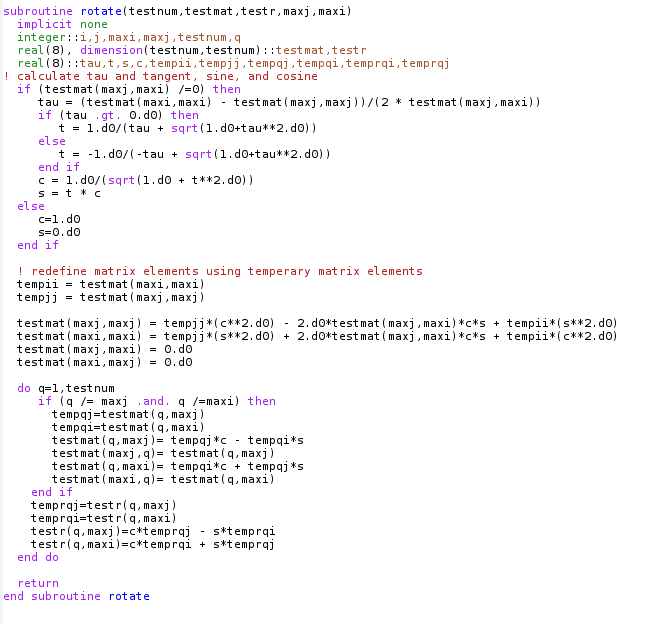
\includegraphics[width=1.2\textwidth]{Rotate.PNG}
    \caption{Code from Jacobi.f90 which implements Jacobi's Algorithm}
\end{figure}

This subroutine is implementing after a separate subroutine searches the matrix to find the largest off diagonal element.  When running Jacobi.f90, the user decides whether to run for 1 or 2 electrons.  The only difference is the potential used.  That can be seen in the code below.

\begin{figure}[H]\label{fig:Potential}
  \centering
    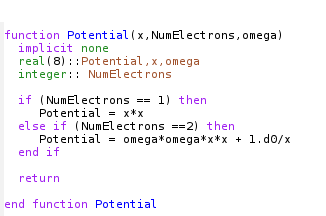
\includegraphics[width=0.8\textwidth]{Potential.PNG}
    \caption{The potential implemented in Jacobi.f90}
\end{figure}

Depending on the user choice, the code will either select the simpler, one electron potential, or the potential for the interacting case.

\subsection{Tests of Code}

This code implements a number of tests to ensue the calculation is working properly.  The first test is doing a test calculation on a 4 by 4 matrix.  The user can choose this option at runtime and Jacobi.f90  will fill a symmetric 4 by 4 matrix with the values:

\begin{equation}
 \begin{bmatrix} 1 & 2 & 3 & 4 \\
                           2 & 6 & 7 & 8 \\
		      3 & 7 & 11 & 12 \\
		     4 & 8 & 12 & 16
             \end{bmatrix}  
\end{equation}

We used Mathematica to produce the exact eigenvalues and eigenfunctions.  After the run, it will print the exact eigenvalues, as well as the computed values.

Additionally, we include a test to check the orthogonality of the transformation.  After every 10 transformations we take the dot product of the two vectors in the eigenvector matrix and check that value is below some tolerance (the value is typically around $10^{-17}$).  If the absolute value of the dot product were to exceed my tolerance, the program would terminate and an error message will print to screen.  The user can choose at runtime whether or not to print these orthogonality checks during the calculation.  The printing will significantly increase the calculation time.

\section{Results and Discussion}


\subsection{Exploring Dependence on Parameters}

The results of the calculation will be sensitive to the choice of $\rho_{max}$ and $N$.  Both of these parameters can be defined by the user while running the program.  We explored the sensitivity to these parameters for the case of the non-interacting electron.  In three dimension, we know the eigenvalues for the three lowest lying, $l=0$ states should be $\lambda_0=3$, $\lambda_1=7$, and $\lambda_2=11$.  Below is a table of convergence for these results for different choices of  $\rho_{max}$ and $N$.

As you can see from the results, $\rho_{max}=6$ and $N=200$ is sufficient for convergence and we used this combination for our runs.

\subsection{Convergence}

\begin{figure}[H]\label{fig:3}
  \centering
    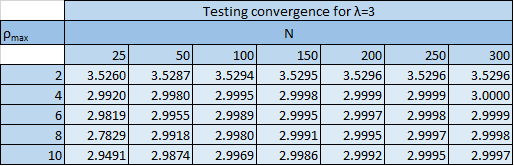
\includegraphics[width=1.1\textwidth]{3.png}
\end{figure}

\begin{figure}[H]\label{fig:7}
  \centering
    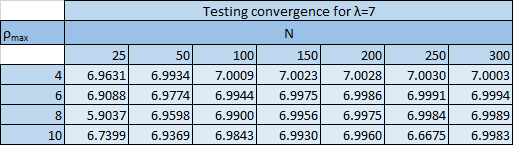
\includegraphics[width=1.1\textwidth]{7.png}
\end{figure}

\begin{figure}[H]\label{fig:11}
  \centering
    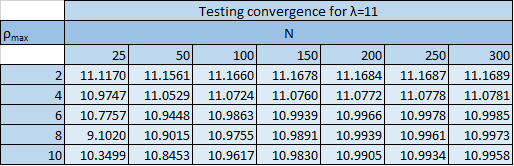
\includegraphics[width=1.1\textwidth]{11.png}
\end{figure}

\subsection{Number of Iterations}

Jacobi's algorithm does not prescribe the necessary number of iterations to zero all off diagonal elements.  To get a sense for this relationship, we ran our code for the case of a single electron for many different matrix sizes, N.  The plot below shows the number of iterations necessary for all off diagonal elements to call below $10^{-8}$.

\begin{figure}[H]\label{fig:iteration}
  \centering
    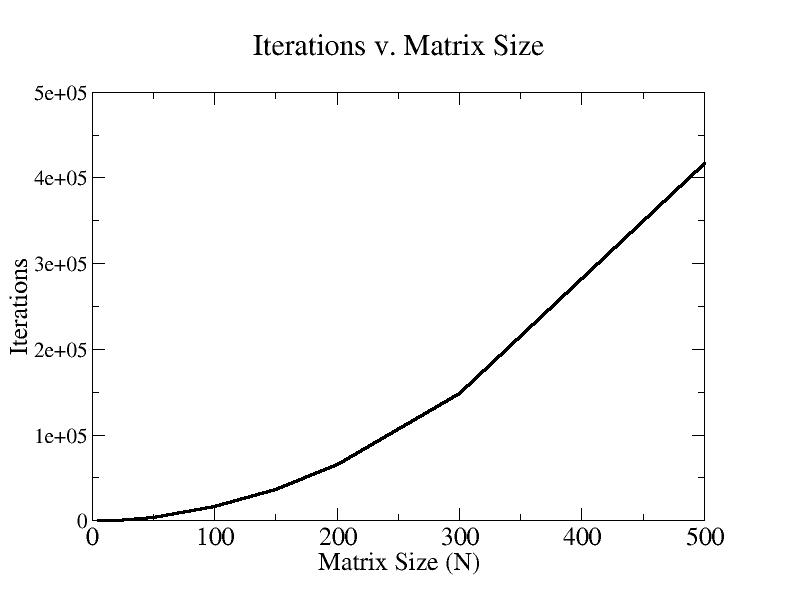
\includegraphics[width=1.1\textwidth]{iterationplot.jpg}
    \caption{Demonstrating the behavior of Iterations v. Matrix Size}
\end{figure}

There does not appear to be a simple relationship between the necessary number of iterations and size of the matrix.  The growth is non-linear, but slower than exponential growth.  A very rough fit in excel found a relatively good fit (by eye) with the second order polynomial $y = 1.7 x^2 - 11.6 x + 116$.  Running for N=1000 took too long for me to obtain a solution, which is unsurprising because, according to this formula, it would require almost 1.7 million iterations.

\subsection{Computational Speeds}

The efficiency of the Jacobi algorithm can be compared to other eigenvalue solvers.  We performed the same calculation using the Linear Algebra PACKage (LAPACK).  Specifically, we used the DSYEV function which produces eigenvalues and eigenvectors for real, symmetric, matrices.  For the case of a non-interacting electron we used both our solver and DSYEV with $\rho_{max}=6$ and $N=200$ and timed both calculations using the cpu\_time function.  DSYEV completed the calculation in 2.18 seconds, while my implementation of Jacobi's algorithm took 7.68 seconds to obtain similar accuracy.

\subsection{Comparing Results to Analytic Results}

For the simple case of two electrons in a harmonic oscillator with l=0, there are some analytic results available.  For this report, we compared my results with M. Taut, Phys. Rev. A, V.48 (1993) \cite{taut}.  Their expressions differ from our development by a factor of $1/2$ so in order to compare, their eigenvalues must be multiplied by two.  For $\omega=0.25$, they obtained a lowest eigenvalue of 0.6250, which should be multiplied by 2 to obtain 1.25.  For $\rho_{max}=10$ and $N=350$, my lowest eigenvalue is 1.2499.  This corresponds to a relative error of $1.28 E^{-5}$

In addition, we varied the value of $\omega$ and studied the effect on the wave functions and eigenvalues.  For these calculations, we ran with $\rho_{max}=10$ and $N=150$.  The results for the eigenvalues are shown in the table below and the eigenfunctions are show in the figure.

\begin{center} 
\begin{tabular}{ |c|c| }
\hline
$\omega$ & $\lambda$ \\
\hline
0.01 & 0.31164 \\
0.5 & 2.23006 \\
1.0 & 4.05761 \\
5.0 & 17.44201\\
\hline
\end{tabular}
\label{table:test}
\end{center}


\begin{figure}[H]\label{fig:compzoom}
  \centering
    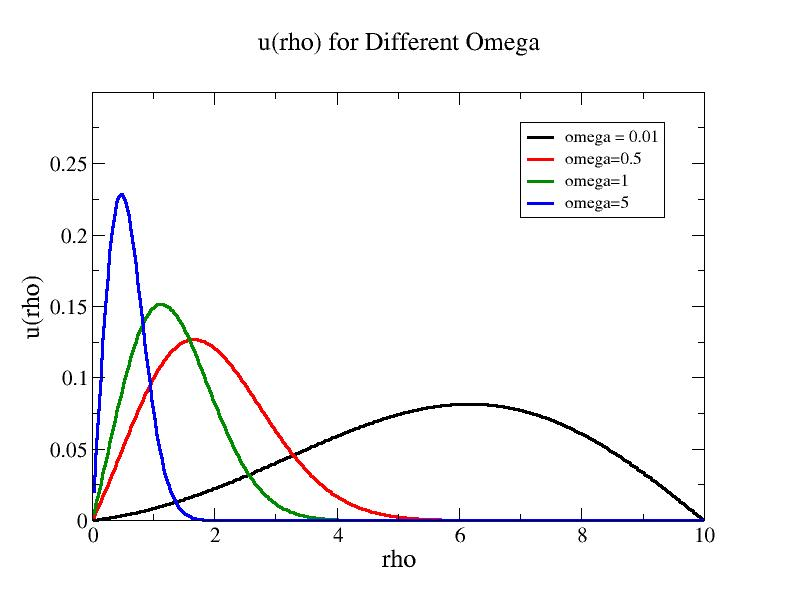
\includegraphics[width=1.2\textwidth]{wavefuntions.jpg}
    \caption{Reduced wave functions for different values of $\omega$}
\end{figure}

As you can see, as $\omega$ increases, the reduced wave function gets pushed in towards the origin.  This can be interpreted as larger values of $\omega$ corresponding to a stronger oscillator well.  In this case, the Coulomb repulsion is overcome by the potential strength, and the electrons being to move into the center of the well.

\section{Conclusions}

In this project we implemented the Jacobi algorithm to solve an eigenvalue problem that describes interacting and non-interacting electrons in a harmonic oscillator.  We tested our code through the implementation of unit tests an comparing results to known values.  For the non interacting case, we were able to reproduce the lowest eigenvalues to a high level of accuracy.  For the interacting case, we were able to reproduce the lowest eigenvalue which can be found analytically.  By studying the eigenfunction we are able to obtain a physical interpretation of $\omega$ where larger values correspond to a tighter oscillator, while larger values correspond to a wider, weaker oscillator.

We also explored the efficiency of the Jacobi algorithm. Time comparisons to eigenvalue solvers showed that Jacobi's method is not particularly efficient.  This is not surprising because there is not prescribed number iterations necessary to complete the transformation.  Additionally, this algorithm does not explicitly take advantage of the tridiagonal nature of the matrix.

\section{Appendices}

\subsection{Appendix A} \label{A}

Consider a basis of orthogonal basis vectors $\mathbf{v}_i$,
\[
\mathbf{v}_i = \begin{bmatrix} v_{i1} \\ \dots \\ \dots \\v_{in} \end{bmatrix}
\]

Orthogonality requires that 

\[
\mathbf{v}_j^T\mathbf{v}_i = \delta_{ij}.
\]

We can apply an orthogonal or unitary transformation such that

\[
\mathbf{w}_i=\mathbf{U}\mathbf{v}_i.
\]

Unitarity enforces that the product of a matrix with its conjugate transpose is the identity matrix.  Orthogonal matrices are a subset of real, unitary matrices.  This condition implies that the product of a matrix with its transpose is the identity matrix.  These two conditions can be expressed as

\[
\mathbf{U}^* \mathbf{U} = \mathbf{U} \mathbf{U}^* = \mathbb{I}
\]

\[
\mathbf{U}^T \mathbf{U} = \mathbf{U} \mathbf{U}^T = \mathbb{I}.
\]

If we now look at the product of our transformed matrix with its transpose, we find

\[
\mathbf{w}^T_j\mathbf{w}_i = (\mathbf{U}\mathbf{v}_i)^T(\mathbf{U}\mathbf{v}_j)= \mathbf{v}_i^T\mathbf{U}^T\mathbf{U}\mathbf{v}_j=\mathbf{v}_i^T\mathbf{U}\mathbf{U}^T\mathbf{v}_j =\mathbf{v}_j^T\mathbf{v}_i = \delta_{ij}.
\]

Therefore, the dot product is preserved.

\begin{comment}

\begin{figure}[H]\label{fig:compzoom}
  \centering
    \includegraphics[width=1.2\textwidth]{compzoom.eps}
    \caption{A zoomed in view of the convergence to the exact solution}
\end{figure}

\begin{center} 
\begin{tabular}{ |c|c|c|c| }
\hline
Size of Matrix ($10^n$) & General & Tailored & LU \\
\hline
1& 3.00 E -6 & 3.00 E -6 & 2.40 E -5\\ 
2 & 4.00 E -6 & 4.00 E -6 & 1.71 E -3 \\ 
3 & 3.90 E -5 & 1.90 E -5 & 1.93\\ 
4 & 3.79 E -4 & 2.09 E -4 & N/A\\ 
5 & 3.38 E -3 & 1.51 E -3  & N/A\\ 
6 & 2.87 E -2 & 1.53 E -2 & N/A\\ 
7 & 3.16 E -1 & 1.73 E -1& N/A\\ 
\hline
\end{tabular}
\label{table:test}
\end{center}

\end{comment}

\begin{thebibliography}{9}

\bibitem{LectureNotes} 
Hjorth-Jensen, Mortehn. 
Computational Physics, Lecture Notes Fall 2015. 
August 2015.


\bibitem{Broida}
Broida, J.
PHYS 130B, Quantum Mechanics II Class Notes.
Fall 2009.
http://www.physics.ucsd.edu/students/courses/fall2009/physics130b/IdentParts.pdf

\bibitem{ClassNotes} 
Taut, M.
Physical Review A, Volume 48, Number 5
November 1993.

\end{thebibliography}



% ------------------- end of main content ---------------

\end{document}

